\newpage

\section{Mathematical model}
\label{sec:math_model}

\begin{figure}[h]
\begin{center}
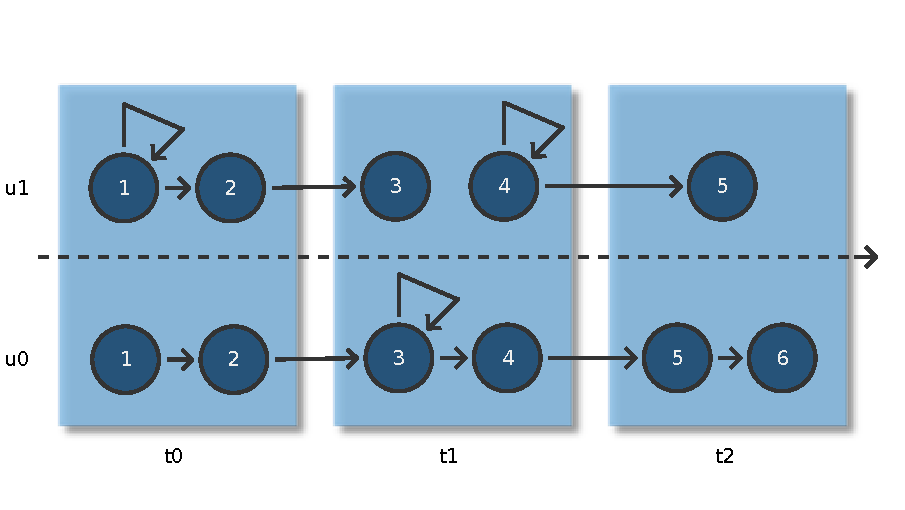
\includegraphics[scale =0.5] {mathematical_definition/images/dynamic_users.pdf}
\caption{Dynamic and static user patterns}
\label{fig:matehematical_model}
\end{center}
\end{figure}


The figure above shows two commuters ${u_0,u_1}$ represented on the vertical axis, grouped by three time windows $t_o,t_1,t_2$. A time window is defined as $t_n$, where $n \in \{0,..,24\}$. Each $t_n$ groups the communications traces of the whole set of commuters in a 60 minutes lapse. 
\\
\\
Let $\vec{P_i} = (p_{ix}, p_{iy})$ be the position vector where $p_{ix}$ is related with the geographic latitud and $p_{iy}$ is related with the geographic longitud of each position.
\\
\\
Formally, a commuter trace during a particular time window and related with a specific user is defined as follows:
$$ T = (\vec{p}_0, \vec{p}_1, ..., \vec{p}_n)  $$ where, 
$\vec{p}_n \in \mathbb{R}^2$ and $n > 1 $.
\\
\\
For instance, regarding with user $0$ and time window $0$ we have the next user trace $ T = (\vec{p}_1, \vec{p}_2)  $. Regarding with user $1$ and time window $0$ we have the next user trace $ T = (\vec{p}_1, \vec{p}_1, \vec{p}_2)  $ and so on.
\\
\\
Also, two functions are defined in order to measure the distance \citep{distance}, given a set of points expressed as spherical coordinates:
$$D(\vec{p}_0, \vec{p}_1) = \text{acos}( \sin(\phi(p_{0x})) * \sin(\phi(p_{1x})) * \cos(\theta(p_{0y}) - \theta(p_{1y})) + \cos(\phi(p_{0x})) * \cos(\phi(p_{1x})))  $$
where:
$$ \phi(x) = (90 - x) * \frac{\pi}{180}$$
$$ \theta(x) = x  * \frac{\pi}{180}$$
therefore the function related to the distance and regarding to a especific user into a temporal window is defined as follows [result in Km]:
$$U = \dysplaystyle 6373 * \sum_{i=0}^{n-1} D(\vec{p}_i, \vec{p}_{i+1}) $$
\\
The second function is related to the number of antenna connections into a trace. The key point is to count only the dynamic transitions, i.e.: remove the self edges over a given trace as follows:
\\
\begin{equation*}
\text{S}(p_0, p_1) = \left \{
\begin{matrix}
0 & \text{if } D(p_0, p_1) = 0 \\
1 & \text{if } D(p_0, p_1) > 0 \\
\end{matrix} \right.
\end{equation*}
therefore, the function regarding to an especific user into a temporal window is defined as follows:
$$N = \dysplaystyle \sum_{i=0}^{n-1} S(\vec{p}_i, \vec{p}_{i+1})$$
